%% ==============================
% Part is used only in PhD thesis
\part{The Implementation}
\chapter{\iflanguage{ngerman}{Implementierung}{Implementation}}
\label{sec:implementation}

\section{Preparation Work}
The concept should later be tested with real hardware at the described in \autoref{c3_sec_used_robots}. The used hardware are KUKA robots and communication with the robots is done via \gls{rsi}. There existed an old driver for the \gls{rsi} as well as a repository with the description of the used robot models.
\subsection{Porting of the KUKA RSI to \gls{ros2} Rolling}
The existing driver for the\gls{rsi} was only available for older versions of \gls{ros} and needed to be ported. 
The driver is implemented as a system and the interfaces of the driver had to be adapted to the signature used in \gls{ros2} Rolling. After the adaption, the drivers have been tested with the robots and some issues where found which needed fixing.\newline 
The first issue discovered was timing related. The control loop of the standard control node in \gls{r2c} consist roughly of five steps as listed in the following:\newline
\lstset{language=C++,basicstyle=\scriptsize}
\begin{lstlisting}[caption=Pseudo code for the control loop.,label=c5_code_control_loop]
// creat controller manager with an rclcpp::executor
auto cm = 
    std::make_shared<controller_manager::ControllerManager>(executor, cm_node_name);
while (rclcpp::ok())
{   
    // step 1: calculated meassured_period
    cm->read(cm->now(), measured_period); // step 2: BLOCKING in RSI driver
    cm->update(cm->now(), measured_period); // step 3
    cm->write(cm->now(), measured_period); // step 4
    //step 5 sleep until next iteration
}
\end{lstlisting}
The communication with the robot controller needs to be neatly timed. The driver creates an UDP server and communicates with the controller of the robot via UDP messages. However, while reading (step 2 in \autoref{c5_code_control_loop}) the new arrived messages from the UDP server, the hardware blocks if no new messages have arrived. Therefore, the update rate set for the control node can get messed up, since the sleep in the blocking read is not preempted. This ultimately leads to the robot controller ending the connection. This problem occurs especially if no real-time kernel is used.\newline
As solution, for the communication with the robot controller the sleep in the control node (step 5 in \autoref{c5_code_control_loop}) is omitted. The synchronization between the robot controller and the controller manager is done via the incoming messages of the robot controller, which acts as clock generator.

A second issue discovered was that the default clock used for the control node does not provide a monotonic increasing time. This leads on platforms where no real-time kernel is installed and especially embedded devices to issues. As a solution, the control node is started with a clock where the time is incremented in monotonic steps as shown in \autoref{c5_code_monotonic_time}
\lstset{language=C++,basicstyle=\scriptsize}
\begin{lstlisting}[caption=Small code extract for setting monotonic clock.,label=c5_code_monotonic_time]
rclcpp::NodeOptions node_options;
node_options.clock_type(rcl_clock_type_t::RCL_STEADY_TIME);
// creat controller manager with an rclcpp::executor
auto cm = std::make_shared<controller_manager::ControllerManager>(executor,
            cm_node_name, node_options);
 // control loop
\end{lstlisting}

\subsection{Restructuring of the \textit{kuka\_experimental} Repo}
The ported \gls{rsi} drivers have then been added to the \textit{kuka\_experimental} repository, which includes the description files of the used robots. The descriptions were updated to include parameters to pass the IP address and port to the driver. Additionally, some restructuring was done to ease the selection and starting of the correct description files. \todo{maybe a bit more}

\section{Adaptions in the \gls{r2c} Framework}
In order to support distributed control of multiple robots in \gls{r2c} a few changes, had to be implemented. In the following first, some preliminary changes are introduced which provide the basis for implementing the proposed concept. Then the changes of the handles and how the controller manager has been adapted are presented.

\subsection{Allow to Start with Empty Robot Description File}
The description of the hardware including which \glspl{ci} and \glspl{si} are provided is normally described in a '\texttt{.xacro}' file. This file is then passed to the controller manager, parsed and the \glspl{ci} and \gls{si} are exported by the hardware. 
As described in \autoref{sec:concept}, a central controller manager does not need to have its own hardware. It imports the \glspl{ci}, \glspl{si} and \glspl{ri} of the sub-controller managers. The problem is, that in \gls{r2c} a controller manager must have its own hardware. In addition, it is not possible to pass the robot description file to the controller manager other than via file at startup. In a distributed setting, it would be an advantage to start a sub-controller manager and then pass the description of the hardware later so that the system is more flexible. \newline
Consequently, the controller manager was changed to allow passing an empty robot description file. The change includes the possibility to now pass the robot description file now over the \textit{~/robot\_description} topic. At construction time it is checked if the robot description file passed to the controller manager is empty. If no robot description is passed via file, it is continued without initializing of the resource manager. The controller manager subscribes to the \textit{~/robot\_description} topic relative to its own private namespaces. This is done to avoid clashes, if multiple controller managers are present, which possibly all get a different hardware passed. The subscription is set to \textit{transient\_local} which is similar to 'latching' publishers in \gls{ros}. This is needed, that a late joining controller manager still gets the description if it has been published, before the controller manager can subscribe to the topic. A code small snippet is presented in \autoref{c5_code_robot_description}.
\lstset{language=C++,basicstyle=\scriptsize}
\begin{lstlisting}[caption=Small code snippet for usage of the robot\_description topic.,label=c5_code_robot_description]
// ControllerManager constructor
{   ...
    if(robot_description.empty()) {
         create_subscription<std_msgs::msg::String>(
        "~/robot_description", rclcpp::QoS(1).transient_local(),
        std::bind(&ControllerManager::robot_description_callback, this,
        std::placeholders::_1));
    } 
    ...
}
// robot_description_callback()
{
    if(!resource_manager->is_urdf_already_loaded()) // check if have been called
    // if not: get urdf, parse, and initialize
}
\end{lstlisting}

\subsection{Activation of Hardware}
After the robot description file has been parsed and the resource manager initialized, the hardware is automatically activated by default. There is no way to configure or activate the hardware components later or  at a specific time. In a distributed setting, this can potentially lead to issues, as a sub-controller manager would instantly activate and start to communicating with its hardware. This should however only be done after the sub-controller manager has registered itself at the central controller manager.\newline
To tackle this, a hardware spawner has been introduced. The hardware spawner is a standalone executable which acts as interface for the \textit{~/set\_hardware\_component\_state} service of the controller manager. It handles service call and allows configuring or activate a hardware component after the resource manager has been initialized and the \glspl{ci} and \glspl{si} have been imported into the resource storage. This way a sub-controller manager can be initialized. Then the \glspl{ci} and \glspl{si} can be created and registered at the central controller. This can now be done before the hardware component is activated and communication with the real hardware started.\newline
The activation can then either be directly in the Python launch file as shown in \autoref{c5_code_hardware_spawning_launch} or via the command line as shown in the \autoref{c5_code_hardware_spawning_cli}. Both examples are activating the
\lstset{language=Python,basicstyle=\scriptsize}
\begin{lstlisting}[caption=Example of using the hardware spawner in a python launch file.,label=c5_code_hardware_spawning_launch]
    hardware_activation = Node(
        package="controller_manager",
        executable="hardware_spawner",
        arguments=["ComponentName", "--activate"],
    )
\end{lstlisting}
fictional hardware component called 'ComponentName'. The only difference is, that with the Python launch file the old behavior is preserved as the hardware is 'automatically' activated at the launch time. Additionally, other nodes can be started timed after the hardware has been successfully activated. What previously was not possible. On the other hand, the hardware can be activated manually from the command line, which was not possible either.
\lstset{
    basicstyle=\fontsize{10}{12}\ttfamily,
    columns=fullflexible,
    language=bash,
    breaklines=true
}
\begin{lstlisting}[caption=Example of using the hardware spawner from command line., label=c5_code_hardware_spawning_cli]
ros2 run controller_manager haelware_spawner "ComponentName" 
    --activate
\end{lstlisting}
\subsection{Adaption of Handles}
As described in \autoref{c4_sec_adaption_of_handles} the \glspl{handle} are the point where the system is split. 
\begin{figure}[htbp]
	\centering
	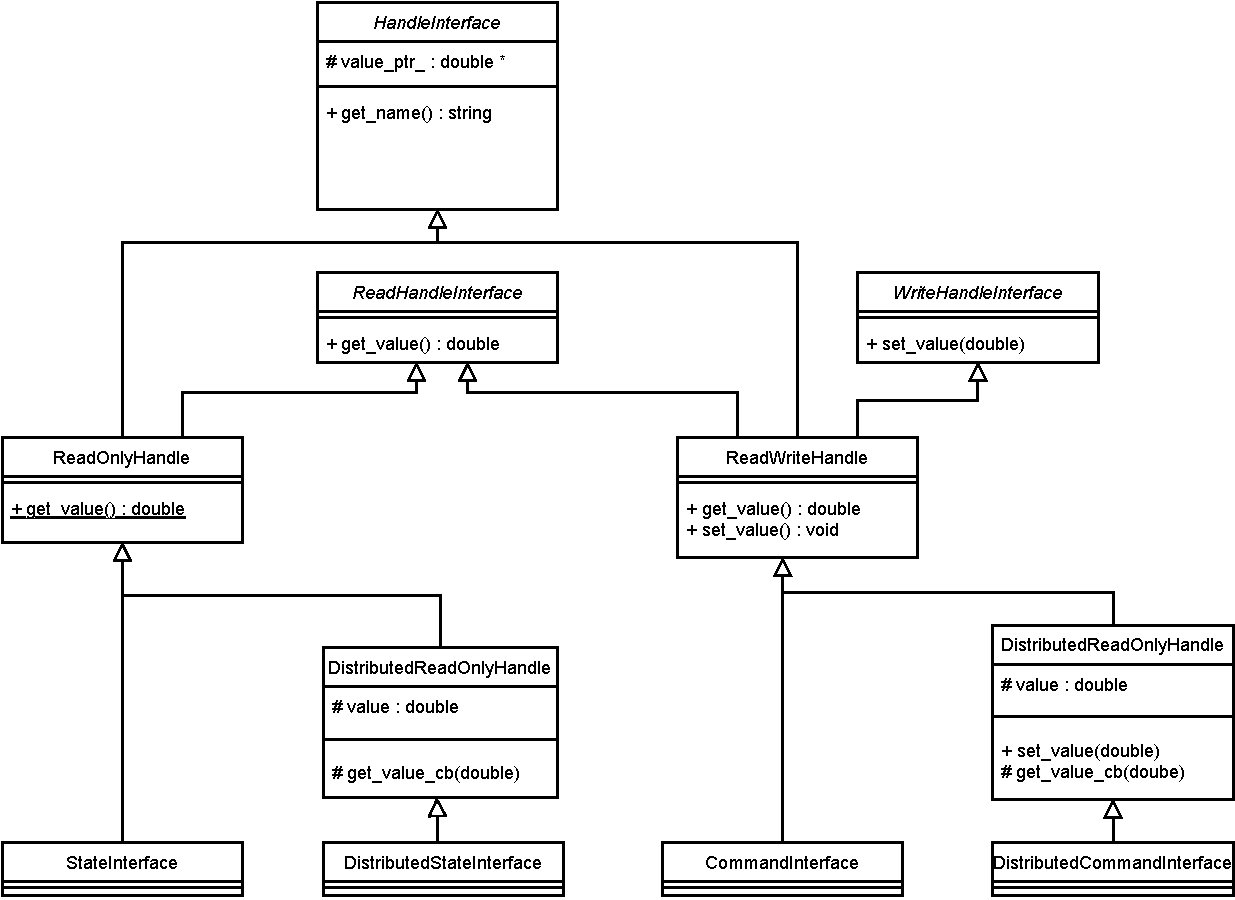
\includegraphics[width=1\textwidth]{Figures/c5/Handles_UML.pdf}
	\caption{UML diagram of the different \gls{handle} types, including the new introduced distributed \glspl{handle}. One should note, that the UML diagram does not contain every member and function of the classes, but only shows the most important parts. }
	\label{c5_fig_handle_uml}
\end{figure}


One problem that arises here is that the \glspl{handle} only store a pointer to the value of the hardware, see \autoref{c3_sec_link_ctrl_hw}. Therefore, the neither a \gls{si} nor a \gls{ci} can know when the value has been changed by the hardware. This poses a problem as in the distributed case the value of the \gls{handle} should be published, if changed. There are two different ways to approach this, each with its own advantages and disadvantages.
\subsubsection*{Publish Value Periodically}
The first approach is to publish the value of the \gls{handle} on timer. One should note, that 
\subsubsection*{Rewrite of the Handles}
\section{Controller Manager Hierarchy}

\subsection{Central Controller Manager}
chainable controller interface
\subsubsection{Configuration of a Central Controller Manager}
\lstset{language=yaml,basicstyle=\scriptsize}
\begin{lstlisting}[caption=Example configuration of a central controller manager with a joint trajecotry controller.,label=c5_l_central_controller_manager_config]
controller_manager:
  ros__parameters:
    central_controller_manager: true
    
    position_trajectory_controller:
      type: joint_trajectory_controller/JointTrajectoryController

position_trajectory_controller:
  ros__parameters:
    joints:
      - /sub_1/sub_1_joint_a1
      - /sub_1/sub_1_joint_a2
      - /sub_1/sub_1_joint_a3
      - /sub_1/sub_1_joint_a4
      - /sub_1/sub_1_joint_a5
      - /sub_1/sub_1_joint_a6
      - /sub_2/sub_2_joint_a1
      - /sub_2/sub_2_joint_a2
      - /sub_2/sub_2_joint_a3
      - /sub_2/sub_2_joint_a4
      - /sub_2/sub_2_joint_a5
      - /sub_2/sub_2_joint_a6

    command_interfaces:
      - position

    state_interfaces:
      - position
    ... # Some configuration for JointTrajectoryController 
\end{lstlisting}

\subsubsection{Configuration of a Chained Central Controller Manager}
\lstset{language=yaml,basicstyle=\scriptsize}
\begin{lstlisting}[caption=Example configuration of a chained central controller manager.,label=c5_l_chained_central_controller_manager_config]
controller_manager:
  ros__parameters:
    central_controller_manager: true

    fpc_jtc_chain_controller:
      type: forward_command_controller/ForwardCommandController

fpc_jtc_chain_controller:
  ros__parameters:
    joints:
      - /sub_1/position_trajectory_controller/sub_1_joint_a1
      - /sub_1/position_trajectory_controller/sub_1_joint_a2
      - /sub_1/position_trajectory_controller/sub_1_joint_a3
      - /sub_1/position_trajectory_controller/sub_1_joint_a4
      - /sub_1/position_trajectory_controller/sub_1_joint_a5
      - /sub_1/position_trajectory_controller/sub_1_joint_a6
      - /sub_2/position_trajectory_controller/sub_2_joint_a1
      - /sub_2/position_trajectory_controller/sub_2_joint_a2
      - /sub_2/position_trajectory_controller/sub_2_joint_a3
      - /sub_2/position_trajectory_controller/sub_2_joint_a4
      - /sub_2/position_trajectory_controller/sub_2_joint_a5
      - /sub_2/position_trajectory_controller/sub_2_joint_a6
    interface_name: position
\end{lstlisting}

\subsection{Sub-Controller Manager}

\subsubsection{Configuration of a Sub-Controller Manager}
\lstset{language=yaml,basicstyle=\scriptsize}
\begin{lstlisting}[caption=Example configuration of a sub-controller manager which exports all of it's command and state interfaces.,label=c5_l_sub_controller_manager_config]
/sub_1/controller_manager:
  ros__parameters:
    update_rate: 10  # Hz
    sub_controller_manager: true
    distributed_interfaces_publish_period: 4 # ms
\end{lstlisting}

\subsubsection{Configuration of a Chained Sub-Controller Manager}
\lstset{language=yaml,basicstyle=\scriptsize}
\begin{lstlisting}[caption=Example configuration of a chained sub-controller manager.,label=c5_l_chained_sub_controller_manager_config]
/sub_1/controller_manager:
  ros__parameters:
    update_rate: 10  # Hz
    sub_controller_manager: true
    distributed_interfaces_publish_period: 4
    export_command_interfaces:
      - ""  # don't export any command interfaces
    export_state_interfaces:
      - "" # don#t export any state intefaces

    position_trajectory_controller:
      type: joint_trajectory_controller/JointTrajectoryController

/sub_1/position_trajectory_controller:
  ros__parameters:
    joints:
      - sub_1_joint_a1
      - sub_1_joint_a2
      - sub_1_joint_a3
      - sub_1_joint_a4
      - sub_1_joint_a5
      - sub_1_joint_a6

    command_interfaces:
      - position

    state_interfaces:
      - position
   ... # Some configuration for JointTrajectoryController 
\end{lstlisting}